\documentclass[addpoints]{exam}

\usepackage{subfigure}
\usepackage{caption}
\usepackage{graphbox}
\usepackage{hyperref}
\usepackage{listings}
\usepackage{multirow}
\usepackage{tabularx}
\usepackage{graphicx}
\usepackage{xcolor}
\usepackage{amsmath}

% Header and footer.
\pagestyle{headandfoot}
\runningheadrule
\runningfootrule
\runningheader{Probability and Statistics}{Final Project}{Spring 2021}
\runningfooter{}{Page \thepage\ of \numpages}{}
\firstpageheader{}{}{}


\title{Final Project}
\author{MATH 310/EE 354 Probability and Statistics\\Habib University\\Spring 2021}
\date{Akeel Ather Medina}

\begin{document}
\maketitle


\section{Random Walk}
\begin{questions}
\question
For this part, we need to take input for the probability, and number of walks. The iteration count has been set to 1000, which means we will end up with 1000 expected final positions.\\
I created an array of size 'iterations' to hold these ending positions, and now for the main calculation, we create a nested loop, of which the inside loop runs 'n' times, and the outer loop runs 'iterations' times. \\
The expected final position is reset to 0 after each walk, and inside the loop, based on the input probability, if we generate a random value from 0 to 1, using np.random.random(), we can determine which way to walk by comparing it to the probability input. \\
The calculation for bins was done, and reused several times in this assignment, using code from stackexchange which is linked in the references tab.\\
This bin width and count is ideal for all situations so value of bins does not need to be changed for different iterations and values of p and n.\\
\\
To begin with, if we plot 100 steps, with the probability of moving along the x-axis as 0.5, given iterations is set to 1000, this is the plot we get:\\
\begin{center}
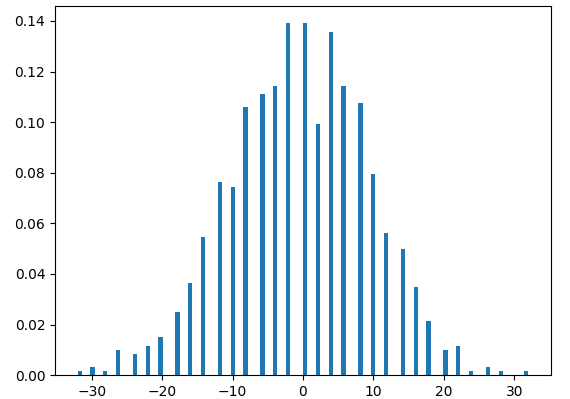
\includegraphics[width=.48\textwidth]{images/p1_1_1.png}
\end{center}
Immediately we can see that this plot follows a normal distribution. Although the expected value does not come out to be 0 every time, it is more likely for it to be nearer to 0 than to be farther away from it. \\
Next we will keep the number of walks similar and test out different probabilities.\\
With $p=0.75$:
\begin{center}
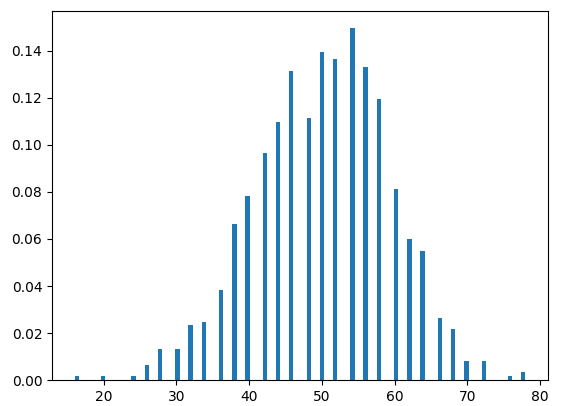
\includegraphics[width=.48\textwidth]{images/p1_1_2.png}
\end{center}
The main difference we can note here is that the mean of our distribution is now around 50, instead of 0. Intuitively speaking, this is because we now have a higher probability of moving to the right, so in 100 steps, if we take 75 to the right and 25 to the left, we will end up on '50'.\\
With $p=0.25$:
\begin{center}
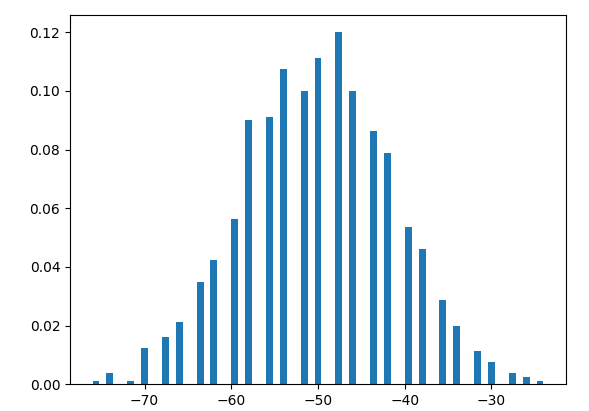
\includegraphics[width=.48\textwidth]{images/p1_1_3.png}
\end{center}
This is a similar situation to the above, but since the probability of moving right is now less likely, out of 100 steps, we will likely move left 75 times, and right 25 times, leaving with an approximate value of 50, as we can see in our plot.\\
With $p=0.99$:
\begin{center}
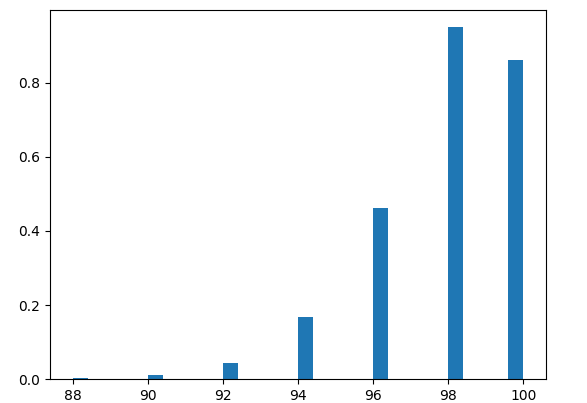
\includegraphics[width=.48\textwidth]{images/p1_1_4.png}
\end{center}

For $p=0.99$ although it does not seem obvious whether this plot follows a normal distribution, the intuitive approach that came to my mind was to increase the number of steps taken. The reason for this is that for such a high probability, with only 100 steps taken a trend cannot be accurately measured because the number of times we will take a step left is very low. Changing the number of steps, although the probability remains the same, gives a chance to observe a normal distribution again because more steps left can be observed. \\Thus this is the plot of $p=0.99$ with $n=1000$.\\
\begin{center}
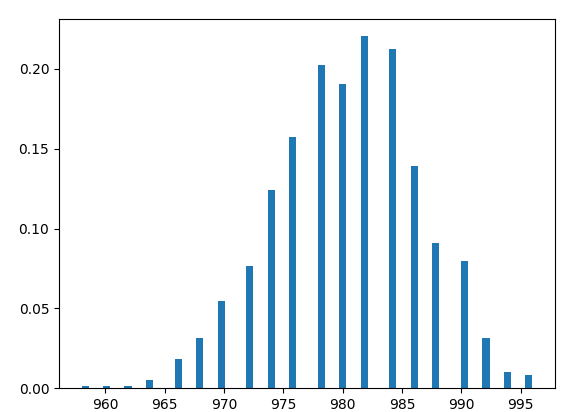
\includegraphics[width=.48\textwidth]{images/p1_1_5.png}
\end{center}

\newpage
\question

For this part, the function is exactly the same except instead of an if-else condition to move left or right, it is now an if-else-if condition, so that in case we are at the point x=1, we cannot move left.\\
The bin width and count is calculated the same way as in the previous part, with a few adjustments to make the trend more obvious.\\
So to highlight the difference with the previous part, I will plot the values in the same order, with n as 100:\\ \\
With $p=0.5$:\\
\begin{center}
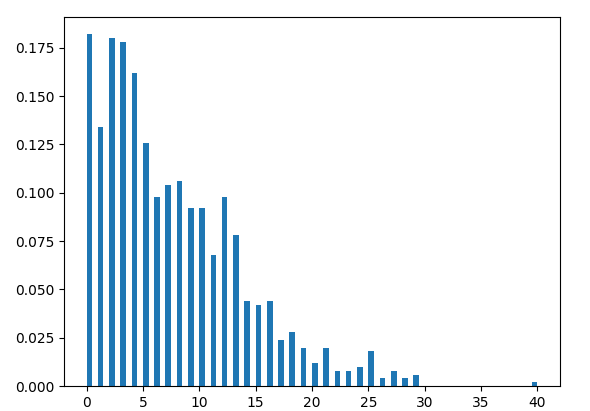
\includegraphics[width=.48\textwidth]{images/p1_2_1.png}
\end{center}
We can immediately see this looks like the right half of the graph we got for part 1. \\
With $p=0.75$:\\
\begin{center}
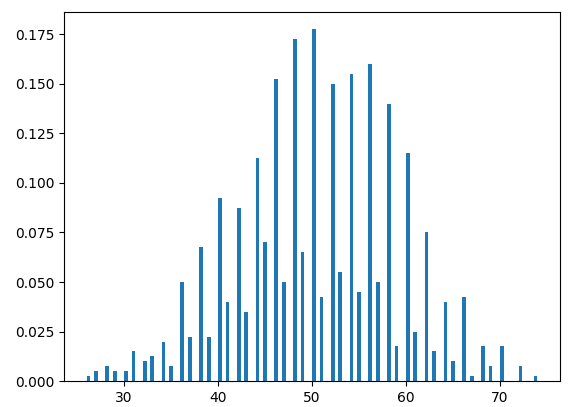
\includegraphics[width=.48\textwidth]{images/p1_2_2.png}
\end{center}
Increasing the probability of moving right leads to the same normal distribution from the last part.\\ \\
With $p=0.25$:\\
\begin{center}
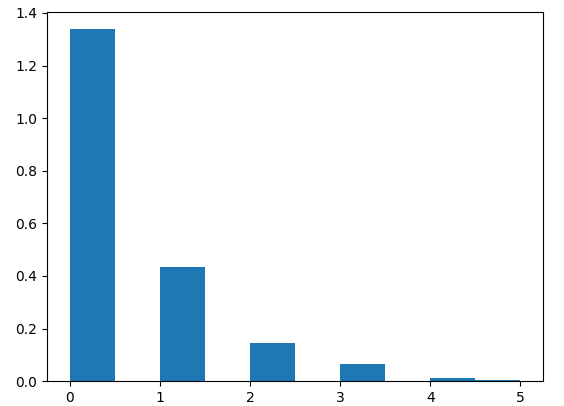
\includegraphics[width=.48\textwidth]{images/p1_2_3.png}
\end{center}
If we were to only consider the positive values from our part 1 equivalent, this plot shows the few positive results we get. In the part 1 equivalent, the mean was near -50, so that is why this graph has such few points plotted, as final values less than 0 are not included.\\ \\
With $p=0.99$:\\
\begin{center}
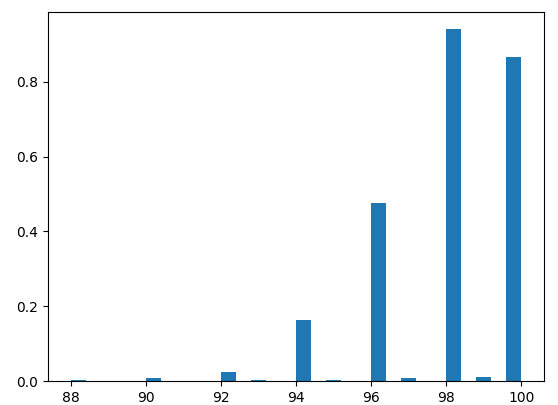
\includegraphics[width=.48\textwidth]{images/p1_2_4.png}
\end{center}
This is identical to our result for the same values in the previous part, so we will continue like before increasing the number of steps, to see if those observations still hold.\\ \\
With $p=0.99$:\\
\begin{center}
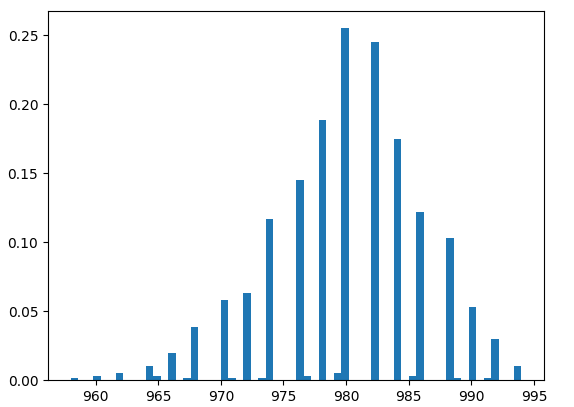
\includegraphics[width=.48\textwidth]{images/p1_2_5.png}
\end{center}
This is very similar to our plot in part 1.\\ \\
With $p=0.25$:\\
\begin{center}
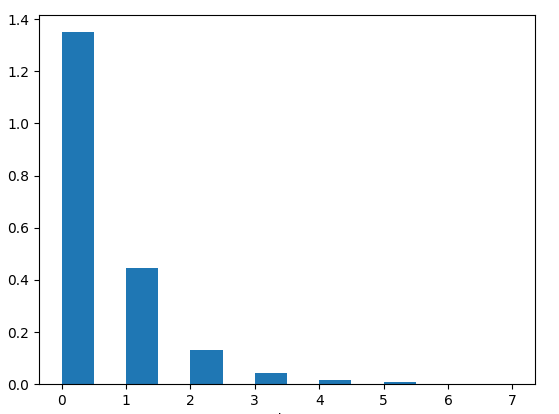
\includegraphics[width=.48\textwidth]{images/p1_2_6.png}
\end{center}
We observe that there is no obvious change for $p=0.25$ even with an increase in steps. This is to be expected because the number of steps would not matter for a normal random variable, the mean and standard deviation would remain the same.

\newpage
\question

For this part we start our code with taking all 4 inputs, the starting point of the objects and the probability they move right. Proceeding with the same approach as in the previous parts, we iterate 'iterations' number of times, and in each iteration, we set the positions of the objects equal to what we previously input. We start a while loop so that only once the objects meet on the real line will the steps be recorded and the next iteration begins. Inside the loop, both objects each move once, and the steps taken for meeting is also incremented.\\
It is important that our starting points have an even distance between them or else it will loop infinitely.\\
The process for determining a right or left step remains the same. First, taking a random value from 0 to 1, and determining if they are less than the probability input, then we move right, else left. Two seperate random values have to be generated for each object.\\
\\
The first plot I tried to compute was for $d1=1$, $d2=-1$, $p1=0.5$ and $p2=0.5$. It was taking too long to compute, but when I tried it again, it worked in just 20 seconds. The plot, however, looked like this:\\
\begin{center}
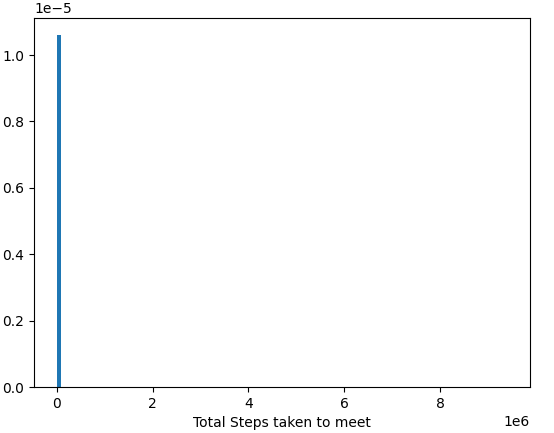
\includegraphics[width=.48\textwidth]{images/p1_3_1.png}
\end{center}
Even after manually adjusting the bins, it was difficult to see all other points, so I printed the max value of the total steps taken, to get 9398093. This value varies greatly, and since there is a much higher probability of the points converging immediately, rather than divering and then converging again, we can only see this one line on the histogram. So i used lines 5-7 from Question 2 part 2 to observe the graph without that cluster of points in the early stage to see if there was a pattern.
\begin{center}
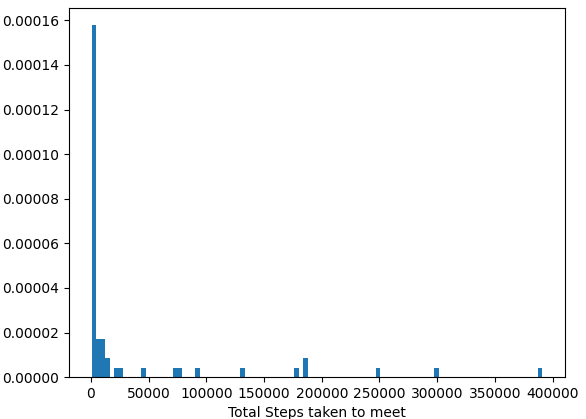
\includegraphics[width=.48\textwidth]{images/p1_3_2.png}
\end{center}
Values lesser than 500 have been removed from our array from which we plot the values. This code has been changed to do the opposite function as that in Question 2 part 2. However, it should be noted that the calculation for bins needs to be commented out when running this, and the argument for the histogram can be arbritrarily assigned, such as to 100. \\
So we can see that for $d1=1$, $d2=-1$, $p1=0.5$ and $p2=0.5$, the steps taken can vary greatly, and the only observation we can make is that for greater total steps, similar results are more sparse. They are clustered together near the beginning. This can be imagined as a graph over time as well. More results are recorded at less 'time' (or steps), and very few the greater the amount of time taken is. There is a lesser probability of steps taken being high.\\ \\
For $d1=1$, $d2=-1$, $p1=0.6$ and $p2=0.6$, the code does not run, and there is a memory error. For different identical values of $p$ as well, such as $0.4$. It is likely that some of the iterations encounter a case where the two objects are chasing after each other and this carries on for too long a time for the computer to compute. \\
\\
For $d1=1$, $d2=-1$, $p1=0.4$ and $p2=0.6$, we get this graph:
\begin{center}
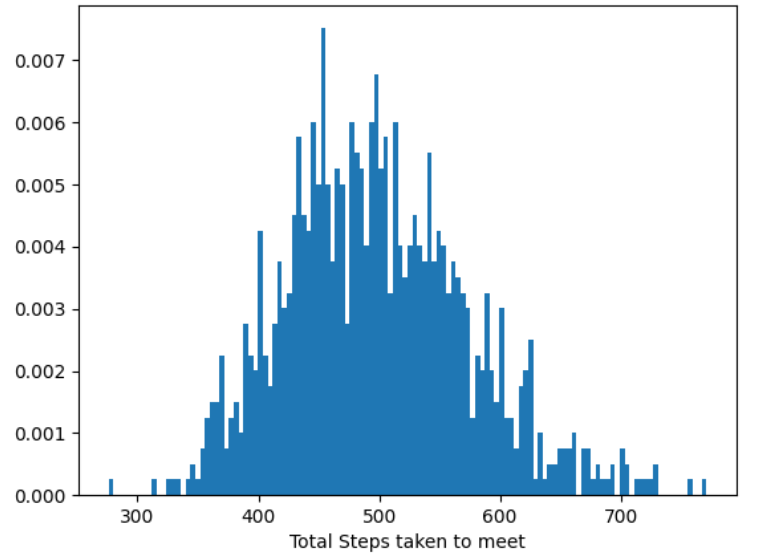
\includegraphics[width=.48\textwidth]{images/p1_3_3.png}
\end{center}
It is obvious that this follows a normal distribution, and so do other plots with a similar nature, such that the probability of the two objects moving together is higher than moving away from each other.
\end{questions}







\newpage
\section{Picking a random point correctly}
\begin{questions}
\question
For this question, I have taken one total input for the radius, which is used by all the parts. Changing the radius has no effect on the graph plotted for all parts.\\
For the first part, since we are now doing a scatter plot, where we need to plot the x and y coordinates of our points, we need 2 different lists to store our values in. To calculate each set of x and y coordinates in the mentioned method asked by the question, in each of 'n' iterations, we randomly calculate a radius, from 0 to the radius limit input by the user, using np.random.uniform. Functionally, this is also identical to the np.random.random function. The angle, $\theta $ is also calculated the same way.\\
To convert this into a plottable set of x and y values we use the formula to convert from polar to cartesian, so $x=r*cos(\theta)$ and $y=r*sin(\theta)$.\\
With iterations set to 50000 for an ideal number of points plotted, each point has a color from the map called 'twilight shifted', which highlights the uniformity of plots, or lack of, which we will see in this part.\\
The code for the plotting of the boundary of the circle was taken from stack exchange.\\
The output of this function looks like:\\
\begin{center}
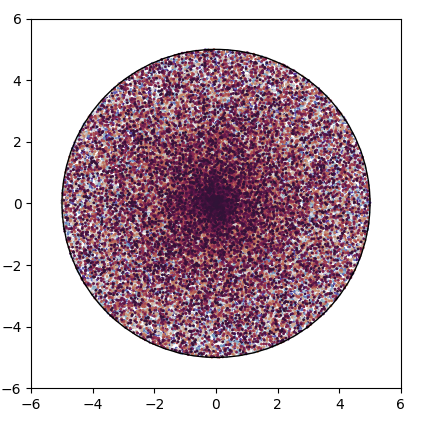
\includegraphics[width=.48\textwidth]{images/p3_1.png}
\end{center}
The scatter plot remains similar for all radius, and the aspect ratio is maintained as a square, with boundaries 1.2 times the diameter of the outer circle. \\
We can see that values closer to the center are more clustered together as compared to ones farther away. The reason for this is that if we compare the area of say half the radius of our outer circle, it will not have half the area. This is because area is determined by $\pi r^2$ and thus is not linear. This means that even if there are an equal amount of points in the inner and outer part of the circle, it will not be uniform because the outer circle has more area to fill, so points are more sparse.\\
Even if we randomly choose radius and $\theta$, the number of plots would have to increase for a higher radius.\\
Another way to think of this is if we take some random angles and draw lines from the origin to the outer circle, then draw points on the intersections of the inner and outer circles, it will seem as if the inner circle has more points because the lines move farther apart the further from the origin we go.\\
\\
The variation of this plot was easily calculated using the np.var function, taking in our list of X coordinates which we use to plot. For 3.1, we get a variation of 0.17 for a radius of 1, and a variation of 4.16 for radius 5.

\newpage
\question
The method for plotting remains the same, the only difference in this part lies in the method of choosing the x and y coordinates. This time, we actually calculate the x and y values in a square of 2*'radius limit'. We randomly choose an x and y coordinate from between the positive and negative values of the input radius, seperately. This is effectively choosing values from a square. We add a while loop so that until the distance of these x and y coordinates from the origin is not within an imaginary circle of specified radius, we keep on choosing new x and y coordinates. This also ensures our data has the same number of elements as compared to the other parts of this question.\\
As with the previous part, the plot remains the same for all kinds of input radius, so this is the output we get:\\
\begin{center}
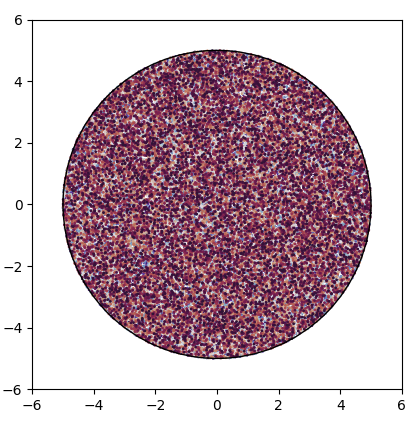
\includegraphics[width=.48\textwidth]{images/p3_2.png}
\end{center}
We can clearly see the difference with the previous part. There is no clustering in the center, and the points are distributed uniformly across the circle. Since we are now uniformly choosing x and y coordinates, it seems likely that given any space on the cartesian plane, sampling x and y coordinates uniformly will give a uniformly filled space. In the previous part, even if we randomly chose radius and $\theta$, the number of plots would have to increase for a higher radius, but over here there is no relation between that and the x and y coordinates. They are independant.\\
\\
The variation of this part using the same function as the previous part gives 0.25 for a radius of 1, and 6.28 for a radius of 5.

\newpage
\question
For this part, we again do the plotting the same way as in the previous parts. The difference lies with how we pick points. In the last part, we found a way to uniformly pick points from a circle using x and y coordinates. In this part, we want to alter our method in the first part, 3.1, which sampled uniformly from polar coordinates instead of cartesian, such that our circle will have points uniformly spread, not clustered in the center. \\
The question first asks that if we plot a circle with radius 1 and a circle with radius 2, is the probability of a point lying in the larger circle 4 times the smaller one in 3.1. This is not the case, since in that part, the radius and angle were chosen randomly. Since a point being within a circle is independent of angle, we know that approximately 50 percent of the time, the radius will be less than 1, and 100 percent of the time it would be lesser than 2. This proves the above question is not true, because the probability of radius being lesser than 2 should be 4 times the probability of it being lesser than 1. \\ \\
We can prove this by using the code created in question 4 for the same reason (to prove that points chosen using 3.2 and 3.3 adhere to this question states above, while 3.1 does not). Using the approach in 3.1, the number of points randomly plotted in a circle of a certain radius, is two times that of a circle with half this radius. However, our approach in 3.2 always gives an approximate value of 4, meaning that a point being the the outer circle is 4 times more likely, thus our approach in that question uniformly picks a point over a circle.\\
Based on this logic, we can try and develop a way of picking radius and angle such that it will be uniformly spread over the circle.\\
So our main goal is to make sure that we calculate our random point in such a way that it has a greater amount of larger values, given we are choosing it uniformly over a range.\\ \\
My first approach was to square random values and accept only if they lie within the radius of the circle, as in part 2, but this also gave a clustered center. \\
My next approach was to randomly pick a value from 0 to the square of the radius, and then take the square root of the answer, however this also resulted in a graph with a clustered center.\\
\\
Next, i ended up using an online source which is the second link in the References tab, for which I tried and ended up getting a uniform distribution. However no explanation was given, so I tried to solve the distribution given as a bonus because I could not guess how to properly choose r and $\theta$ to get random points uniformly, and ended up with:\\
\begin{center}
$k = \frac{1}{\pi r^2} $\\
$P(r \leq R) = \frac{1}{R^2}*r^2$\\
$\sqrt{P(r \leq R)} = \frac{r}{R}$\\
\end{center}
What I figured from this is that to choose a random point in the circle, we need to take the square root of the probability of it lyring inside a circle fo radius r $\leq$ R, and multiply it with the radius R itself. Since the probability is between 0 and 1, this makes sense as the square root of numbers lesser than 1 gives a value greater than itself (as shown in 4.4), or in other words, further from the center. Since we want a random point inside our circle, the main line of code seperating this approach from 3.1 is:\\
\begin{center}
$np.sqrt(np.random.random()) * radiuslimit$\\
\end{center}
This line of code is similar to the line I saw in the online source. The graph plotted for this formula for choosing a point, similar to 3.2, looks like:\\
\begin{center}
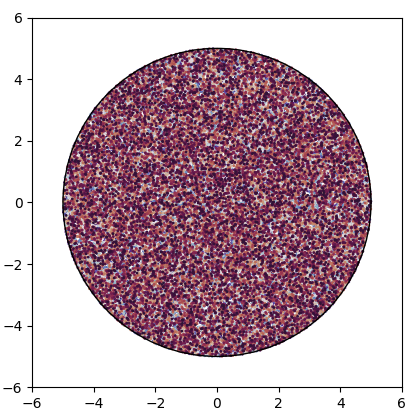
\includegraphics[width=.48\textwidth]{images/p3_3.png}
\end{center}

The variation of X coordinates for a radius of 1 is 0.25, and 6.25 for radius 5. The variance of X coordinates in 3.2 and 3.3 is approximately the same.

\end{questions}



\newpage
\section{Saying random is not enough}
\begin{questions}
\question
In this question, we need to randomly generate 2 angles between 0 and 2*pi, and the chord length is the distance between the two points of where the angle extends to touch the circle. If we calculate this for any two arbritary angles, we could imagine it as a triangle being formed with two sides being of length 'radius', and the last side being the chord length. To calculate this chord length we can divide the triangle into two halves, and apply basic trigonometry to get the chord length. That is:\\
\begin{equation}
 c = 2 * r * \sin{(|a2-a1|/2)}
\end{equation}
Where c is the length of the chord, a1 and a2 are the angles randomly chosen each iteration, and r is the radius. We divide the angle by 2 because we can only apply $\sin(\theta) = \frac{Opposite}{Hypotenuse}$ if we have a right triangle, which we can do by splitting the triangle we form with angle $|a2-a1|$ into 2 parts. This only gives half the chord length, so multiplying by two gives our final chord length. \\
\\
The plot of chord length generated by this formula looks like: \\
\begin{center}
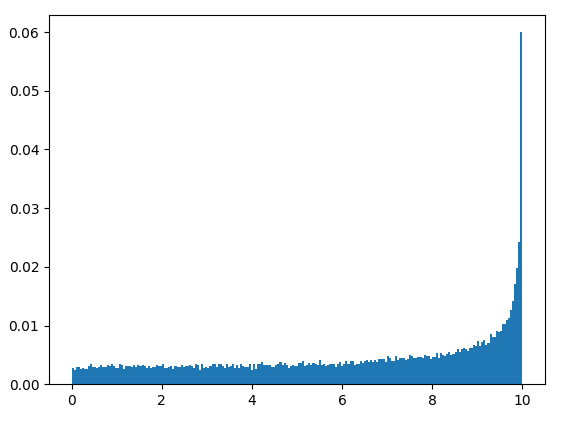
\includegraphics[width=.48\textwidth]{images/p4_1_1.png}
\end{center}
Note that bin calculation remains the same as in previous parts. The only difference is that we have set the y axis to plot probability of occurrance. \\
We can see that the highest probability of chord length is that for it being approximately 10, then greately decreasing. The radius for all questions was chosen as 5. This means that the angles being 180 degrees apart is the most likely scenario, as when the angles are 180 degrees apart, the chord between them will give us a length of 10 for this circle. We can confirm this, as if for example angle 1 is 180 and angle 2 is 0, we will do sin(90) which gives 1. Thus our final answer will be 10, the maximum chord length.
\newpage
\question
In this second approach, we need to choose a random angle, and randomly pick a point from the angle extended to the boundary of the circle, from the origin. This point will be the perpendicular bisector of some chord, and that is how we choose it. Now one thing to note is that when calculating the chord length, we do not actually need the angle. This is because the chord length can simply be calculated using pythogoras theorem. We know this perpendicular bisector meets two points of the circle, and any point on the circle to the origin is of length radius. Next, we ourselves are choosing this random point from 0 to radius, thus we also know the length of the line from the origin to the point, and the origin to the point on the circle where the bisector cuts. Thus, by manipulating pythogoras theorem we get:\\
\begin{equation}
 c = \sqrt{r^2 - p^2}
\end{equation}
Where r is the radius, and p is the random point on the line. However, as we noticed in the last question, choosing a random point from 0 to the radius (as the questions asks us to), we will not get a uniform distrubution of points on this circle. As proof, I assigned 2 variables as counters for our points generated, if these points (they are not x and y points, but a polar radius) are lesser than radius (as all of them must be, giving a number the same as 'iterations), increment the variable called outer by 1, and if they are lesser than $\frac{radius}{2}$, then increment inner by 1. The reason for doing it this way is it is the example given to us in 3.3. If we have two circles, one of double the radius, it should have 4 times the amount of area (or points plotted inside it). This code works for any radius and any number of iterations, and we always approximately get an output of 2, when we compute $\frac{outer}{inner}$. This shows that the center of the circle is more clustered and has more points than the outer circle.\\
Back to the question, our distribution of chord lengths looks like:\\
\begin{center}
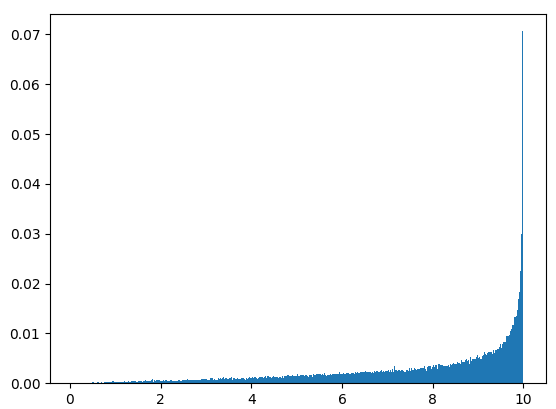
\includegraphics[width=.48\textwidth]{images/p4_2_1.png}
\end{center}
We can see the difference with this and the last part. There are very few chords with a small length, and many with a higher length. The reason could be as shown before, that points with a location nearer to the origin will have a much larger chord length than to the edge.
\newpage
\question
For this question, to pick a random point uniformly from a circle i re-used my code from 3.2, in which a random x and random y value is chosen from the square of side 'radius', until it is physically within a circle of radius 'radius'.  
The code is otherwise identical to the previous part. For our calculation of the point in the circle, we need it in terms of radius so that we can apply the same pythogorean manipulation as before. The formula for this is:\\
\begin{equation}
 p = \sqrt{x^2 + y^2}
\end{equation}
Where p is the 'radius', in cartesian to polar form. \\
I have commented out the approach used in 3.3 for a random point as an alternative approach, it also gives the same plot.\\
The difference in this part and the previous part can be seen by our results of inner and outer at the end of our iterations, this time $\frac{outer}{inner}$ always gives an approximate value of 4, as compared to 2. This is how we know that our point being chosen is uniform over our circle. Our distribution looks like:\\
\begin{center}
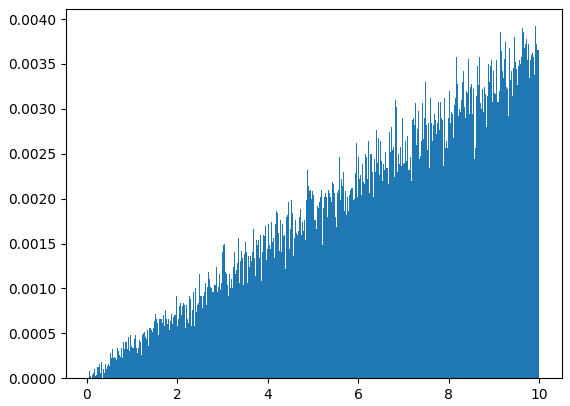
\includegraphics[width=.48\textwidth]{images/p4_3_1.png}
\end{center}
This distrubution looks widely different from the previous ones. It is linearly decreasing, with the most chord lengths being of maximum length possible. I will elaborate on why I think this approach is the most accurate in the next part.\\
\newpage
\question
Our approach in 4.3 intuitively should give the most accurate random chord length, the reason being that it is the only part where the points chosen are also uniform over a circle, not biased like in 4.2. A possible explanation for the nature of our plot in 4.3 could be that, for example, if we consider a circle of radius 1. Now lets use our way of calculating chord length. For the points 0.1, 0.2, 0.5, 0.9: \\
\begin{center}

$\sqrt{1^2 - 0.1^2} = 0.995$    \\
$\sqrt{1^2 - 0.2^2} = 0.980   $   \\
$\sqrt{1^2 - 0.5^2} = 0.866     $   \\
$\sqrt{1^2 - 0.9^2} = 0.436 $    \\
\end{center}
The result does not decrease linearly, and thus our final plot, although the chord lengths are random, is not greatest for values in our 'outer circle', although now the outer circle has 4 times the amount of points as the inner. Also we should note that our approach in 3.3 has made sure this holds for all radius, as the distribution is between 0 and 1, multipied by a constant, the max radius.
\end{questions}


\newpage
\section{References}

\noindent\fbox{%
    \parbox{\textwidth}{%
\url{https://stackoverflow.com/questions/33203645/how-to-plot-a-histogram-using-matplotlib-in-python-with-a-list-of-data}{The code for calculation of bins for all histograms was taken from here.}\\
\url{https://blogs.sas.com/content/iml/2016/03/30/generate-uniform-2d-ball.html}{Referred to a line of code on this website for 3.3}
    }%
}


\end{document}
